
\de{ĐỀ THI GIỮA HỌC KỲ I NĂM HỌC 2022-2023}{THPT Bình Chiểu - Đề 125}

\begin{bt}%[Dự án đề kiểm tra GHKI NH22-23- Quan Ổn]%[0T1Y3-1]%Câu 1:
	Cho $A=\{2; 3; 4; 5; 6\}$; $B=\{0; 3; 4; 6; 7\}$. Tìm $A \cap B, A \cup B$.
	\loigiai{
		Ta có $A\cap B=\{3;4;6\}$ và $A\cup B=\{0;2;3;4;5;6;7\}$.
	}
\end{bt}

\begin{bt}%[1,5 điểm]%Nguyễn Hữu Hiệp - Phan Thanh Tâm%[0T1B3-2]%Câu 2:
	Cho $A=(6;9] ; B=[4;+\infty)$. Tìm $A \cap B, A \cup B, C_{\mathbb{R}} A$.
	\loigiai{
		Ta có  $A\cap B=(6;9]$, $A\cup B=[4;+\infty)$ và $\mathrm{C}_{\mathbb{R}}A=(-\infty;6]\cup(9;+\infty)$. 
	}
\end{bt}

\begin{bt}%[Dự án đề kiểm tra GHKI NH22-23- Quan Ổn]%[0T2B1-2]%Câu 3:
	Biểu diễn miền nghiệm của bất phương trình sau trên mặt phẳng tọa độ: $3x+y<9$.
	\loigiai{
		\immini{
			Đường thẳng $\Delta\colon 3x+y=9$ đi qua hai điểm $A(0;9)$ và $B(3;0)$.\\
			Thay $x = 0$ và $y = 0$ vao bất phương trình, ta được $0 < 9$ (luôn đúng) nên điểm $O(0;0)$ thuộc miền nghiệm của bất phương trình $3x+y<9$.\\
			Kết luận: Miền nghiệm của bất phương trình là phần không gạch chéo, không chứa đường thẳng $\Delta$.
		}{
			\begin{tikzpicture}[scale=0.4, line join=round, line cap=round, >=stealth]
				\tikzset{every node/.style={scale=0.8}}
				\def\xmin{-1}\def\xmax{5}\def\ymin{-1}\def\ymax{10}
				\draw[->] (\xmin-0.2,0)--(\xmax+0.2,0) node[below] {$x$};
				\draw[->] (0,\ymin-0.2)--(0,\ymax+0.2) node[right] {$y$};
				\draw (0,0) node [below left] {$O$};
				\foreach \x in {3}\draw (\x,0.1)--(\x,-0.1) node [below left] {$\x$};
				\foreach \y in {9}\draw (0.1,\y)--(-0.1,\y) node [left] {$\y$};
				\clip (\xmin,\ymin) rectangle (\xmax,\ymax);
				\fill [pattern=north east lines,pattern color=blue!20] plot[smooth,samples=200,domain=\xmin:\xmax](\x,{-3*(\x)+9})--
				(\xmax,\ymin)--(\xmax,\ymax);
				\draw[thick,smooth,samples=200,domain=\xmin:\xmax] plot (\x,{-3*(\x)+9});
				\draw (0,9)--(3,0)node[pos=0.6,above,sloped]{$\Delta\colon 3x+y=9$};
				\fill (0,9) circle (1pt);
				\fill (3,0) circle (1pt);
			\end{tikzpicture}
		}
	}
\end{bt}

\begin{bt}%[Dự án đề kiểm tra GHKI NH22-23- Quan Ổn]%[0T2K2-2]%Câu 4:
	Một học sinh trường THPT Bình Chiểu dự định gấp hạc và làm hoa để đem bán gây quỹ từ thiện giúp đỡ một học sinh trong trường mắc bệnh hiểm nghèo. Cần 4 phút để gấp 1 con hạc và 5 phút để làm được 1 bông hoa. Biết 1 con hạc bán giá $5.000$ đồng, 1 bông hoa bán giá $8.000$ đồng và học sinh này có không quá 80 phút để làm. Tổng số sản phẩm không vượt quá 18. Hỏi bạn cần làm bao nhiêu sản phẩm mỗi loại để thu được nhiều tiền nhất?
	\loigiai{
		\immini{
			Gọi $x$, $y$ lần lượt là số con hạc và số bông hoa cần làm $(x,y\geq 0)$.\\
			Số tiền thu được sau khi bán: $F(x,y)=5x+8y$ (nghìn đồng).\\
			Theo đề bài, ta có hệ bất phương trình $$\heva{&4x+5y\le80\\&x+y\le18\\&x\ge0\\&y\ge0.}$$
			Miền nghiệm của hệ là miền tứ giác $OABC$, kể cả biên với các đỉnh lần lượt là $O(0;0)$, $A(0;16)$, $B(10;8)$, $C(18;0)$.
		}{
			\begin{tikzpicture}[scale=0.3, line join=round, line cap=round, >=stealth]
				\tikzset{every node/.style={scale=0.9}}
				\def\xmin{-2}\def\xmax{22}\def\ymin{-2}\def\ymax{20}
				\draw[->] (\xmin-0.2,0)--(\xmax+0.2,0) node[below] {$x$};
				\draw[->] (0,\ymin-0.2)--(0,\ymax+0.2) node[right] {$y$};
				\clip (\xmin,\ymin) rectangle (\xmax,\ymax);
				\fill [pattern=north east lines,pattern color=gray] (\xmin,0)--(\xmax,0)--
				(\xmax,\ymin)--(\xmin,\ymin);
				\fill [pattern=north east lines,pattern color=gray] (0,\ymin)--(0,\ymax)--(\xmin,\ymax)--(\xmin,\ymin);
				\fill [pattern=north east lines,pattern color=red!20] plot[samples=20,domain=\xmin:\xmax] (\x,{-1*(\x)+18})--(\xmax,\ymin)--(\xmax,\ymax)--(\xmin,\ymax);
				\fill [pattern=north east lines,pattern color=blue!20] plot[samples=20,domain=\xmin:\xmax] (\x,{-4/5*(\x)+16})--(\xmax,\ymin)--(\xmax,\ymax)--(\xmin,\ymax);
				\draw (0,0) node [above right] {$O$};
				\foreach \x in {10,18,20}\draw (\x,0.1)--(\x,-0.1) node [below] {$\x$};
				\foreach \y in {8,16,18}\draw (0.1,\y)--(-0.1,\y) node [left] {$\y$};
				\clip (\xmin,\ymin) rectangle (\xmax,\ymax);
				\draw[thick,smooth,samples=200,domain=\xmin:\xmax] plot (\x,{-1*(\x)+18});
				\draw[thick,smooth,samples=200,domain=\xmin:\xmax] plot (\x,{-4/5*(\x)+16});
				\draw (0,16)node[right]{$A$}(10,8)node[above right]{$B$} (18,0)node[above]{$C$};
				\draw[dashed] (10,0)--(10,8)--(0,8);
			\end{tikzpicture}
		}
		\noindent Ta có $F(0,0)=0$, $F(0,16)=128$, $F(10,8)=114$ và $F(16,0)=80$.\\
		Vậy số tiền thu được nhiều nhất là 128.000 đồng khi gấp được 0 con hạc và 16 bông hoa.
	}
\end{bt}

\begin{bt}%[Dự án đề kiểm tra GHKI NH22-23- Quan Ổn]%[0T3B1-2]%Câu 5:
	Tìm tập xác định của các hàm số sau
	\begin{multicols}{2}
		\begin{enumerate}[a)]
			\item $y=\dfrac{2x}{x^2-8x+15}$.
			\item $y=\sqrt{3x-15}$.
		\end{enumerate}
	\end{multicols}
	\loigiai{
		\begin{enumerate}[a)]
			\item Điều kiện $x^2-8x+15\ne0\Leftrightarrow \heva{&x\ne5\\&x\ne3.}$\\
			Vậy tập xác định của hàm số $y=\dfrac{2x}{x^2-8x+15}$ là $\mathscr{D}=\mathbb{R}\setminus\{3;5\}$.
			\item Điều kiện $3x-15\ge0\Leftrightarrow x\ge5$.\\
			Vậy tập xác định của hàm số $y=\sqrt{3x-15}$ là $\mathscr{D}=[5;+\infty)$.
		\end{enumerate}
	}
\end{bt}

\begin{bt}%[Dự án đề kiểm tra GHKI NH22-23- Quan Ổn]%[0T3B2-3]%Câu 6:
	Khảo sát sự biến thiên và vẽ đồ thị của hàm số $y=x^2+4x-1$.
	\loigiai{
		\immini{
			\begin{itemize}
				\item Đỉnh $I(-2;-5)$.
				\item Trục đối xứng $x=-2$.
				\item Bảng biến thiên:
				\begin{center}
					
\begin{tikzpicture}
						\tkzTabInit[nocadre=false,lgt=1.2,espcl=2,deltacl=0.6]
						{$x$/0.6,$y$/2}{$-\infty$,$-2$,$+\infty$}
						\tkzTabVar{+/$+\infty$,-/$-5$,+/$+\infty$}
					\end{tikzpicture}
				\end{center}
				\item Hàm số đồng biến trên $(-2;+\infty)$, hàm số nghịch biến trên $(-\infty;-2)$.
				\item Bảng giá trị
				\begin{tabular}{c|c|c|c|c|c}
					$x$ & $-4$ & $-3$ & $-2$ & $-1$ & $0$ \\
					\hline
					$y$ & $-1$ & $-4$ & $-5$ & $-4$ & $-1$\\
				\end{tabular}
				\item Đồ thị
			\end{itemize}
		}{
			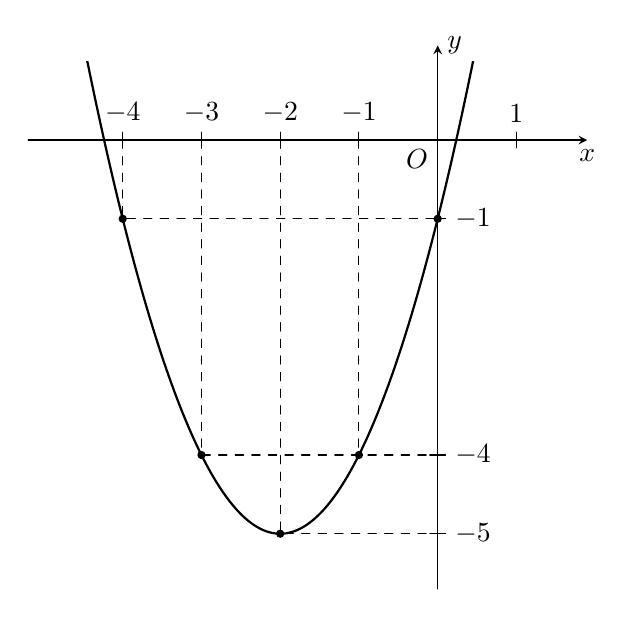
\begin{tikzpicture}[scale=1, line join=round, line cap=round, >=stealth]
				\tikzset{every node/.style={scale=1}}
				\def\xmin{-5}\def\xmax{1.7}\def\ymin{-5.5}\def\ymax{1}
				\draw[->] (\xmin-0.2,0)--(\xmax+0.2,0) node[below] {$x$};
				\draw[->] (0,\ymin-0.2)--(0,\ymax+0.2) node[right] {$y$};
				\draw (0,0) node [below left] {$O$};
				\foreach \x in {-4,-3,-2,-1,1}\draw (\x,-0.1)--(\x,0.1) node [above] {$\x$};
				\foreach \y in {-1,-4,-5}\draw (-0.1,\y)--(0.1,\y) node [right] {$\y$};
				\clip (\xmin,\ymin) rectangle (\xmax,\ymax);
				\draw[thick,smooth,samples=200,domain=\xmin:\xmax] plot (\x,{1*((\x)^2)+4*\x-1});
				\draw[dashed] (-4,0)--(-4,-1)--(0,-1);\fill (-4,-1) circle (1.5pt);
				\draw[dashed] (-3,0)--(-3,-4)--(0,-4);\fill (-3,-4) circle (1.5pt);
				\draw[dashed] (-2,0)--(-2,-5)--(0,-5);\fill (-2,-5) circle (1.5pt);
				\draw[dashed] (-1,0)--(-1,-4);\fill (-1,-4) circle (1.5pt);
				\fill (0,-1) circle (1.5pt);
			\end{tikzpicture}
		}
	}
\end{bt}

\begin{bt}%[Dự án đề kiểm tra GHKI NH22-23- Quan Ổn]%[0T3B2-2]%Câu 7:
	Xác định các hệ số $a$ và $b$ của hàm số bậc hai $y=ax^2+bx-2$. Biết đồ thị hàm số đi qua điểm $A(1;7)$ và có trục đối xứng $x=-1$.
	\loigiai{
		Đồ thị hàm số đi qua điểm $A(1;7)$ suy ra $a+b=9$.\\
		Đồ thị hàm số có trục đối xứng $x=-1$ suy ra $-\dfrac{b}{2a}=-1\Leftrightarrow 2a-b=0$.\\
		Ta có hệ phương trình $\heva{&a+b=9\\&2a-b=0}\Leftrightarrow \heva{&a=3\\&b=6.}$
	}
\end{bt}